\documentclass{standalone}
\usepackage{tikz}
\usetikzlibrary{shapes.geometric, arrows.meta, positioning}
\definecolor{blockcolor}{RGB}{63, 72, 204}
\definecolor{arrowcolor}{RGB}{0, 162, 232}

\begin{document}
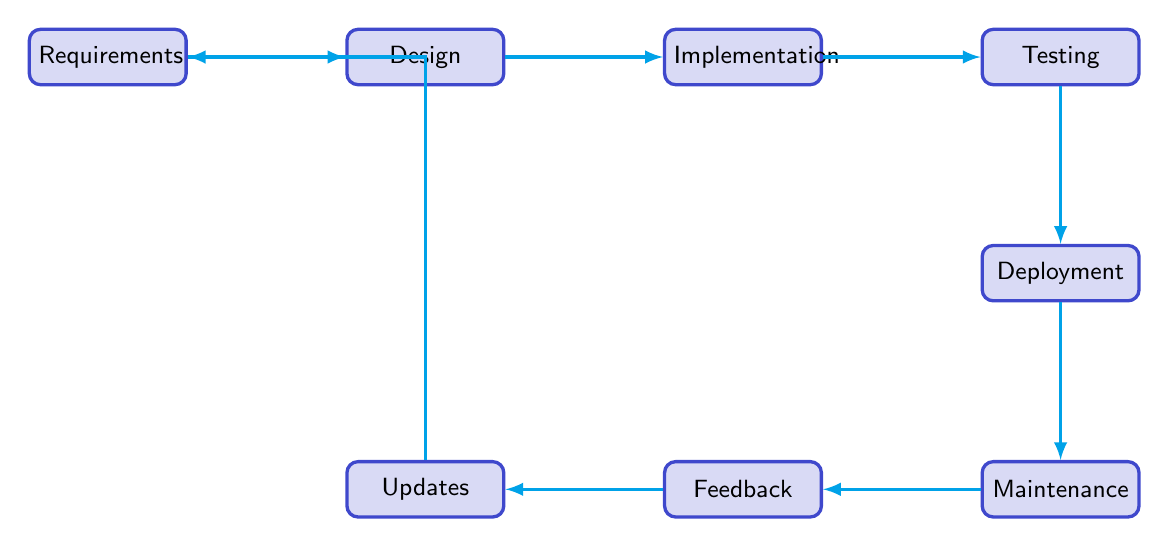
\begin{tikzpicture}[
  node distance = 2cm,
  auto,
  font=\sffamily,
  block/.style = {
    rectangle,
    rounded corners,
    draw = blockcolor,
    fill = blockcolor!20,
    very thick,
    text width = 5em,
    align = center,
    minimum height = 2em
  },
  arrow/.style = {
    ->,
    >=latex,
    draw = arrowcolor,
    very thick
  },
  every node/.style={
    font=\sffamily\small
  }
]

% Nodes
\node[block] (requirements) {Requirements};
\node[block, right=of requirements] (design) {Design};
\node[block, right=of design] (implementation) {Implementation};
\node[block, right=of implementation] (testing) {Testing};
\node[block, below=of testing] (deployment) {Deployment};
\node[block, below=of deployment] (maintenance) {Maintenance};
\node[block, left=of maintenance] (feedback) {Feedback};
\node[block, left=of feedback] (updates) {Updates};

% Arrows
\draw[arrow] (requirements) -- (design);
\draw[arrow] (design) -- (implementation);
\draw[arrow] (implementation) -- (testing);
\draw[arrow] (testing) -- (deployment);
\draw[arrow] (deployment) -- (maintenance);
\draw[arrow] (maintenance) -- (feedback);
\draw[arrow] (feedback) -- (updates);
\draw[arrow] (updates) |- (requirements);

\end{tikzpicture}
\end{document}
